\documentclass[12pt,pdftex,a4paper]{article}
\usepackage[ngerman]{babel}
\usepackage[utf8]{inputenc}
\usepackage{amsmath}
\usepackage{amssymb}
\usepackage{ulem}
\usepackage{bbm}
\usepackage{array}
\usepackage{marvosym}
\usepackage{color}
\usepackage{hhline}
\usepackage[pdftex]{graphicx}
\usepackage{listings}
\lstset{language=Python,basicstyle=\footnotesize}
\usepackage{pdfpages}
\usepackage{booktabs}
\PassOptionsToPackage{hyphens}{url}
\usepackage{hyperref}
\usepackage{extarrows}
\usepackage{rotating}
\usepackage{dsfont}
\usepackage{circuitikz}
\newcommand\tab[1][1cm]{\hspace*{#1}}

\usepackage{fancyhdr}
\pagestyle{fancy}
\lhead{Franziska Hutter(3295896) - 
	Felix Truger(3331705) - 
	Felix Bühler(2973410)}
\renewcommand{\headrulewidth}{0.6pt}

\title{Security and Privacy,\\ Blatt 5}
\author{Franziska Hutter (3295896)\\
	Felix Truger (3331705)\\
	Felix Bühler (2973410)}


\begin{document}
\maketitle
\pagebreak

\section*{Problem 1: Schnorr’s protocol - special honest verifier zero-knowledge}

% SEE for reference: http://www.cs.au.dk/~ivan/Sigma.pdf
% https://cs.nyu.edu/courses/spring07/G22.3220-001/lec2.pdf
% danieleventuri.altervista.org/files/zero-knowledge.pdf (contains proof)

It is easy to see, that $(P, V)$ as given for Schnorr’s protocol has the form of a $\Sigma$-protocol with commitment $a$, challenge $e$ and response $z$.
The ``special honest verifier ZK'' property requires: $\exists$ ppt simulator $M$ such that $\forall x\in L_R$ and $e\in \{0,1\}^t: M(x, e) = Trans_{V^e}^P(x)$ where $Trans_{V^e}^P(x)$ is the Transcript of an interaction between $P$ and $V$ using challenge $e$ on input $x$.
\\~\\to be continued

\section*{Problem 2: Homomorphic properties of algorithms}
$p=(\mathcal{G},q,g,h)$ fixed, $r_0, r_1, v_0, v_1 \in \mathbb{Z}_q$, we show:
$$com^{r_0+r_1}(p, v_0 + v_1) \overset{!}{=} com^{r_0}(p, v_0) \cdot com^{r_1}(p, v_1)$$
By just applying the definition of $com$ in the Pedersen commitment scheme, we know:
$$com^{r_0+r_1}(p, v_0 + v_1) = g^{v_0 + v_1}\cdot h^{r_0+r_1}$$
$$com^{r_0}(p, v_0) = g^{v_0} \cdot h^{r_0}$$
$$com^{r_1}(p, v_1) = g^{v_1} \cdot h^{r_1}$$
Thus:
$$com^{r_0}(p, v_0) \cdot com^{r_1}(p, v_1) = g^{v_0} \cdot h^{r_0} \cdot g^{v_1} \cdot h^{r_1}$$
$$= g^{v_0}\cdot g^{v_1}\cdot h^{r_0}\cdot h^{r_1}$$
$$= g^{v_0 + v_1}\cdot h^{r_0+r_1}$$
$$= com^{r_0+r_1}(p, v_0 + v_1)$$

% This definitely seems TOO EASY?!?

\section*{Problem 3: Building circuits for functions}
Find the drawing of our circuit for $f$ below.\\
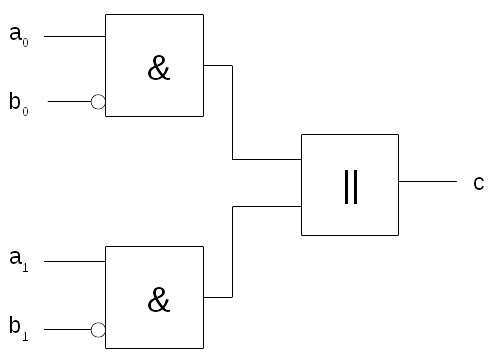
\includegraphics[width=200pt]{./problem3_binary_circuit.png}

\section*{Problem 4: Garbled circuits}
Find a garbled circuit for the given circuit below.\\
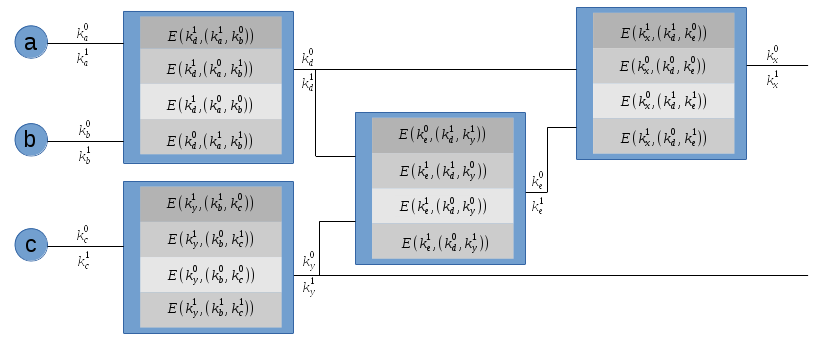
\includegraphics[width=\textwidth]{./problem4_garbled_circuit.png}

\section*{Problem 5: 51\%-Attack on Bitcoin}

\end{document}